\section{Aufbau und Durchführung}
\label{sec:Durchfuehrung}
In Abbildung 5 ist der Aufbau der Strahlenquelle und des Zählrohrs schematisch dargestellt. Es wird ein Geiger-Müller-Zählrohr, das an ein
elektrisches Zählwerk angeschlossen ist, in einer Linie mit einer Strahlenquelle angeschlossen. Dazwischen
lässt sich ein Absorbermaterial befestigen und sowohl das Zählrohr als auch die Quelle sind mit Blei abgeschirmt.
\begin{figure}
    \centering
    \label{fig:Aufbau}
    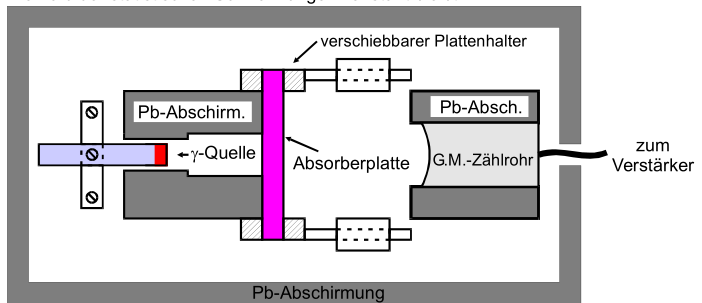
\includegraphics{Bilder/Aufbau.png}
    \caption{Schematischer Versuchsaufbau der Strahlenquelle und des Zählrohrs\cite{sample}.}
\end{figure}
Zu Beginn wird für $t=900\,\unit{s}$ eine Nullmessung durchgeführt, um die Hintergrundstrahlung zu ermitteln.
Als $\gamma$-Strahler wird $^{137}$Cs verwendet und für Eisen und Blei mit unterschiedlichen Dicken gemessen. Für den
$\beta$-Strahler wird $^{99}$Tc verwendet und für unterschiedliche Dicken von Aluminium gemessen.